\section{MÉTODOS}
\label{sec:metodos}

%%%%%%%%%%%%%%%%%%%%%%%%%%%%%%%%%%%%%%%%%%%%%%%%%%%%%%%%%%%%%%%%%%%%%%%%%%%%%%%
\subsection{Aquisição dos dados}
\label{subsec:aquisi_dado}
\par{Foi construinda um fluxo de requisição de dados com python utilizando a biblioteca \textit{obspy} para acessar o banco de dados \textit{MOHO} e obter 60 segundos de forma de onda a partir de 10 segundos antes do seleção de onda 'P' e que a origem preferida do epicentro estivesse a pelo menos 400 km de distancia da estação que foi realizada o pick. Por tanto, todos os eventos que foram rotulados, porém estivesse a mais de 400km ou não possuisem a seleção da onda 'P' foram descartados.
}

%%%%%%%%%%%%%%%%%%%%%%%%%%%%%%%%%%%%%%%%%%%%%%%%%%%%%%%%%%%%%%%%%%%%%%%%%%%%%%%
\subsection{Testes e validação do Classificador}
\label{subsec:testes_validacao}
\par{O classificador foi testado utilizando um conjunto de dados rigorosamente selecionado, composto por eventos rotulados como naturais por especialistas. Esta fase de testes foi crucial para validar a precisão do classificador na discriminação entre eventos antrópicos e naturais, ajustando parâmetros e refinando o modelo conforme necessário.}

\par{Os resultados dos testes foram encorajadores, mostrando uma boa capacidade do modelo em identificar corretamente a natureza dos eventos sismológicos. As métricas de desempenho, como precisão e recall, foram calculadas e apresentaram resultados satisfatórios, reforçando a eficácia do classificador desenvolvido.}

\par{Adicionalmente, foram realizados ajustes baseados nos resultados dos testes, incluindo a otimização da captura de dados e do pré-processamento, para melhorar a acurácia das classificações.}

%%%%%%%%%%%%%%%%%%%%%%%%%%%%%%%%%%%%%%%%%%%%%%%%%%%%%%%%%%%%%%%%%%%%%%%%%%%%%%%
\subsection{Análise de Eventos em Horários Não Comerciais}
\label{subsec:nao_comerciais}

%
\begin{figure}[ht!]
	\captionsetup{justification=justified, singlelinecheck=false, width=1\textwidth}
    \caption{Mapa do Brasil mostrando pontos de interesse e os epicentros dos eventos classificados como detonações e sismos. Foram detectados um total de sessenta e sete (67) eventos associados a detonações no período, classificados a partir do horário de ocorrência e da forma de onda, além do plano de fogo fornecido, com magnitudes mínima e máxima de 0.4 e 3.0 MLv, respectivamente.}
    \begin{mdframed}[
        linecolor=black,
        linewidth=1pt,
        roundcorner=10pt,
    ]
    \begin{center}
    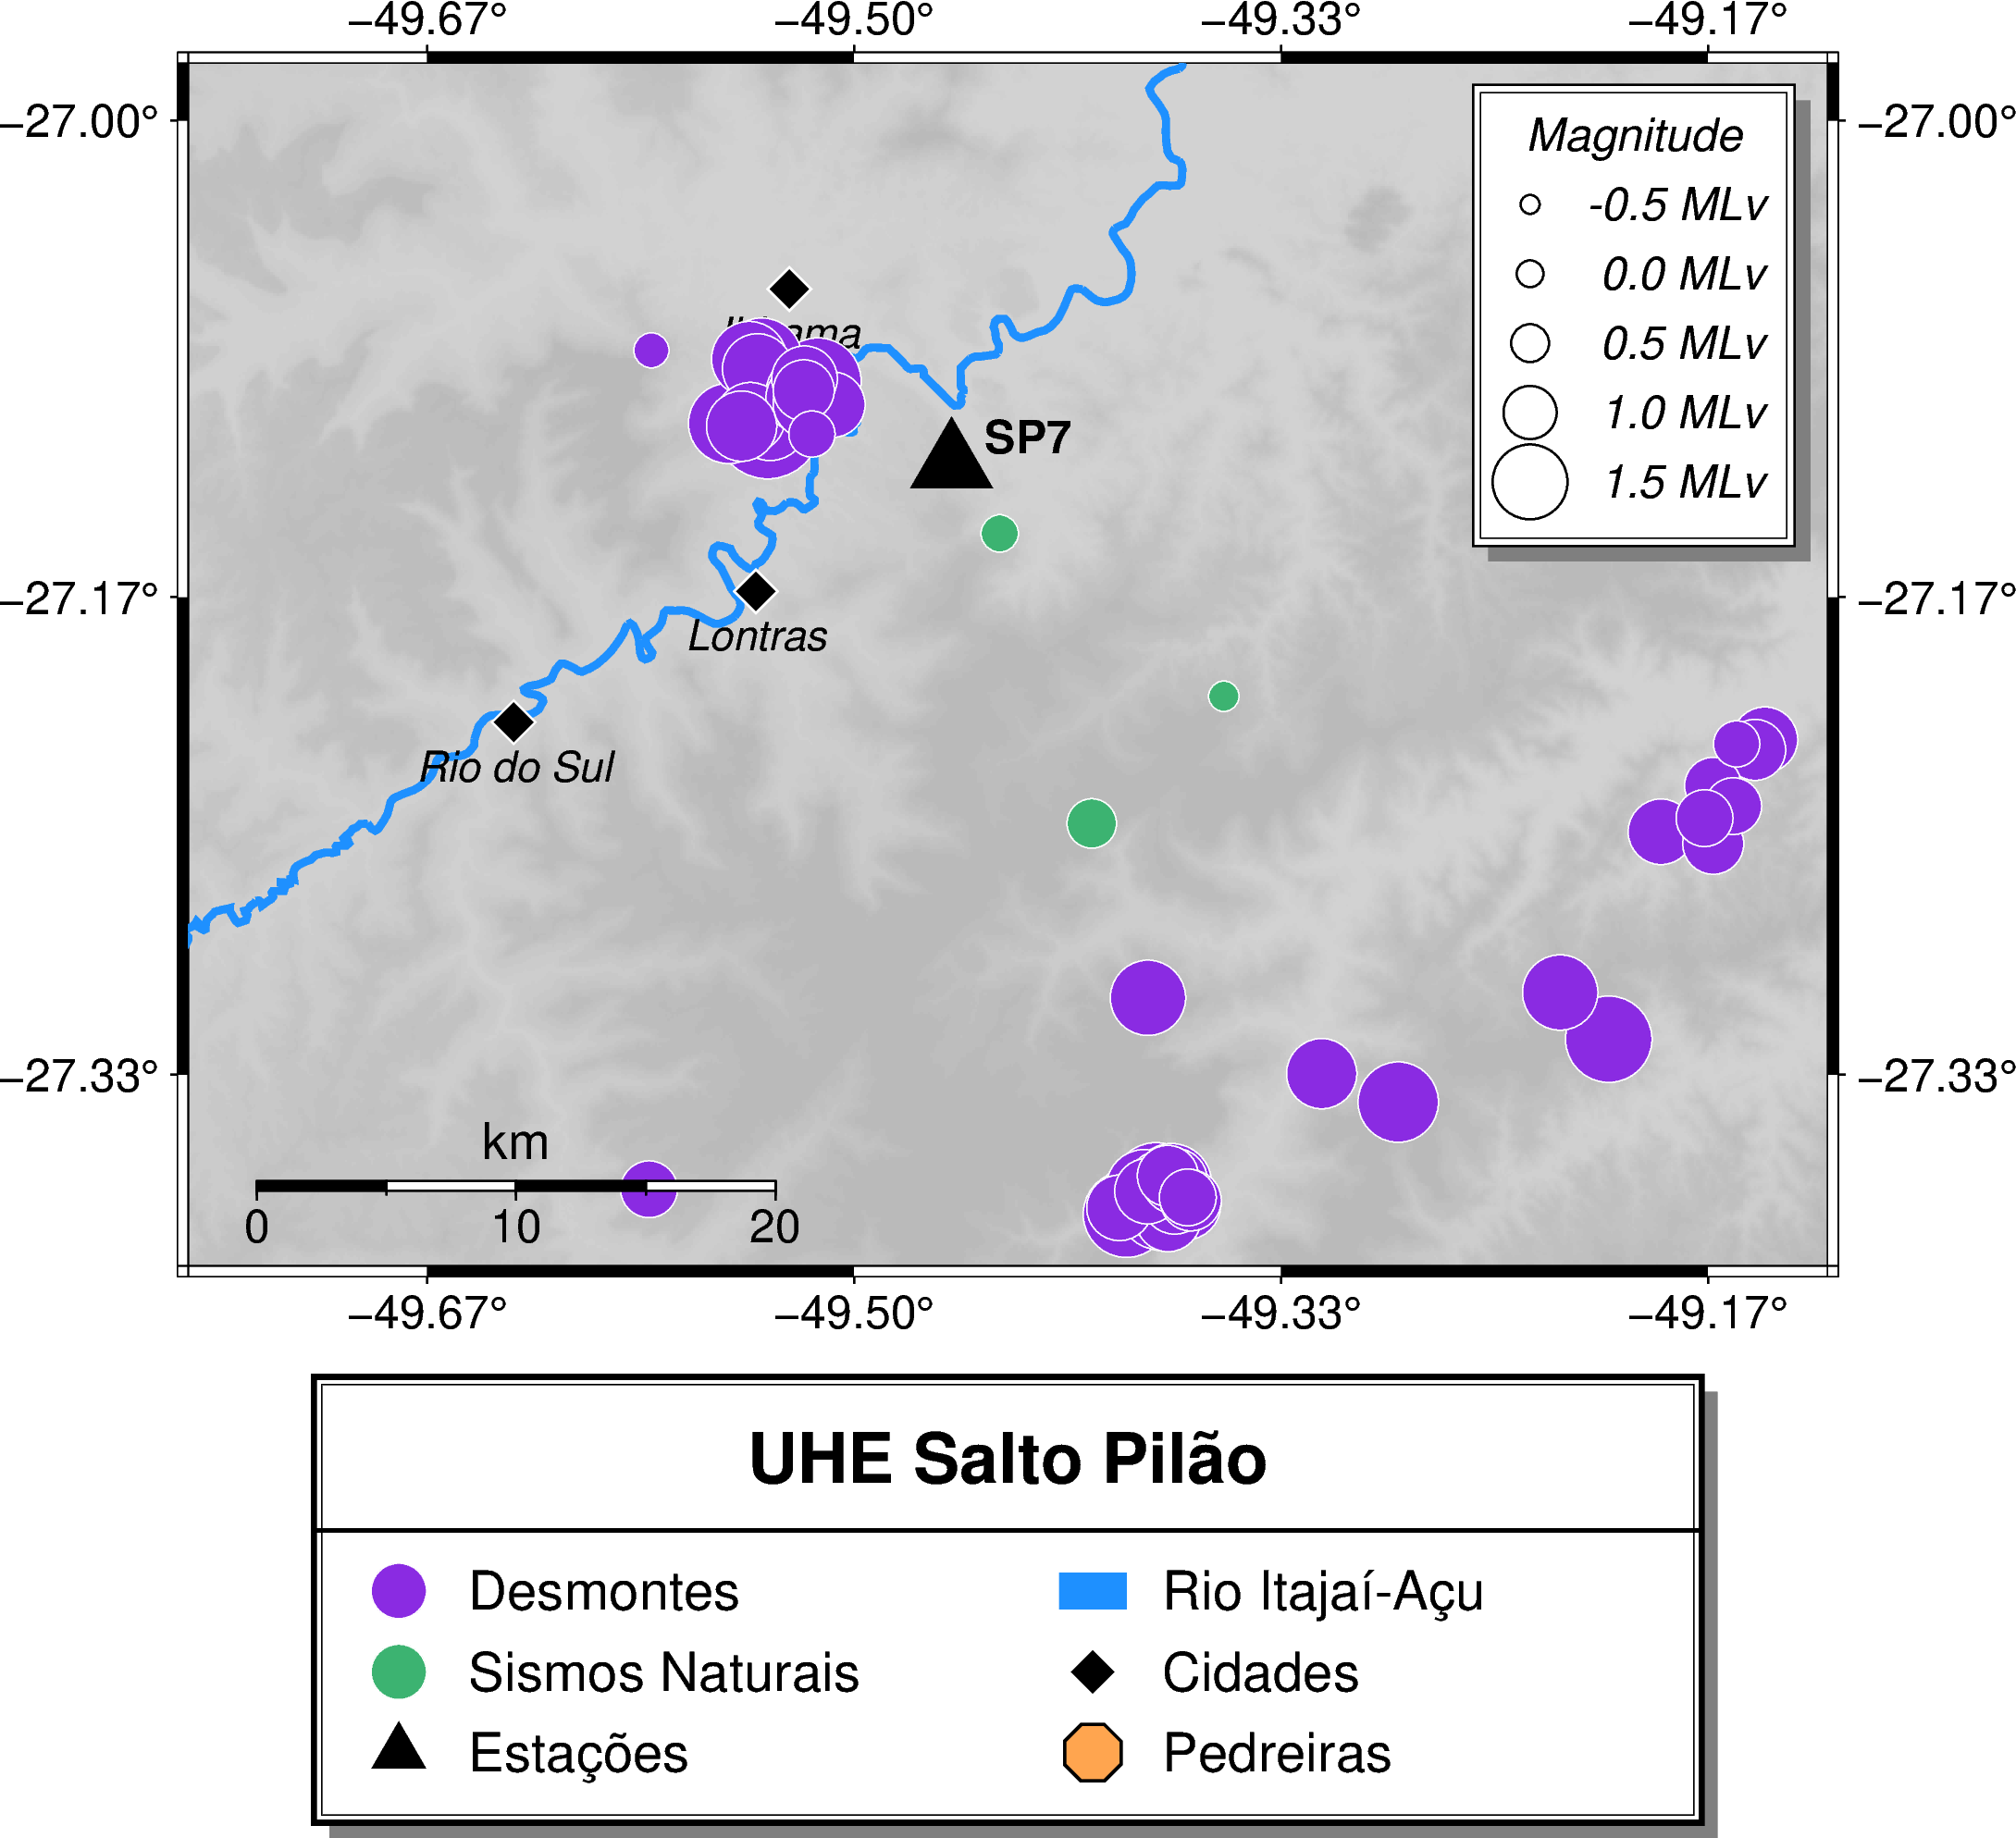
\includegraphics[width=0.8\textwidth]{/home/ggrl/projetos/ClassificadorSismologico/arquivos/figuras/mapas/mapa.png}
    \end{center}
    \end{mdframed}
    \caption*{Fonte: IPT}
\end{figure}


\par{Uma parte significativa do estudo envolveu a análise de eventos sismológicos registrados em horários não comerciais, definidos como o período entre as 23:00 UTC e 11:00 UTC. Este intervalo foi escolhido considerando as diferenças de fuso horário entre as várias regiões do Brasil, que abrangem de -3 UTC a -5 UTC. A análise focou em identificar características distintivas dos eventos naturais e antropogênicos ocorridos neste período.}

\par{Os dados foram processados e visualizados usando uma série de scripts Python desenvolvidos para filtrar, analisar e plotar informações sismológicas detalhadas. Os gráficos resultantes, como distribuições de probabilidade natural, boxplots de distância por natureza do evento e matrizes de correlação, ajudaram a ilustrar diferenças significativas nas características dos eventos registrados durante o horário não comercial.}

\par{Especificamente, a distribuição de \textit{prob\_nat} (probabilidade de um evento ser natural) para eventos naturais mostrou-se distinta daquela para eventos antropogênicos, com eventos naturais tendendo a ter valores mais altos de probabilidade. Além disso, a análise de recall por número de estações envolvidas no registro dos eventos revelou que um maior número de estações frequentemente correlaciona-se a uma classificação mais precisa entre eventos naturais e antropogênicos.}

\par{Os histogramas de recall ajustados para a hora do dia destacaram a precisão da classificação durante os horários não comerciais, refletindo a eficácia do algoritmo em identificar corretamente a natureza dos eventos sob condições variáveis de ruído ambiental e atividade humana.}

\par{Todas essas análises são cruciais para entender a dinâmica sismológica em horários menos típicos para atividades humanas, oferecendo insights sobre a influência de fatores naturais isolados das interferências antrópicas. Os resultados estão detalhados nos Apêndices A e B, onde figuras e tabelas fornecem uma representação visual e quantitativa das descobertas.}

\par{A validação destes resultados foi facilitada pela utilização de scripts automatizados que permitiram uma reprodutibilidade eficiente e a geração de outputs consistentes para análises subsequentes e revisões de estudo.}

\par{Este foco em eventos durante períodos não comerciais não apenas enriquece a compreensão da sismicidade natural mas também aprimora as metodologias de monitoramento e análise sismológica em condições controladas de ruído.}
